% Template for Elsevier CRC journal article
% version 1.2 dated 09 May 2011

% This file (c) 2009-2011 Elsevier Ltd.  Modifications may be freely made,
% provided the edited file is saved under a different name

% This file contains modifications for Procedia Computer Science

% Changes since version 1.1
% - added "procedia" option compliant with ecrc.sty version 1.2a
%   (makes the layout approximately the same as the Word CRC template)
% - added example for generating copyright line in abstract

%-----------------------------------------------------------------------------------

%% This template uses the elsarticle.cls document class and the extension package ecrc.sty
%% For full documentation on usage of elsarticle.cls, consult the documentation "elsdoc.pdf"
%% Further resources available at http://www.elsevier.com/latex

%-----------------------------------------------------------------------------------

%%%%%%%%%%%%%%%%%%%%%%%%%%%%%%%%%%%%%%%%%%%%%%%%%%%%%%%%%%%%%%
%%%%%%%%%%%%%%%%%%%%%%%%%%%%%%%%%%%%%%%%%%%%%%%%%%%%%%%%%%%%%%
%%                                                          %%
%% Important note on usage                                  %%
%% -----------------------                                  %%
%% This file should normally be compiled with PDFLaTeX      %%
%% Using standard LaTeX should work but may produce clashes %%
%%                                                          %%
%%%%%%%%%%%%%%%%%%%%%%%%%%%%%%%%%%%%%%%%%%%%%%%%%%%%%%%%%%%%%%
%%%%%%%%%%%%%%%%%%%%%%%%%%%%%%%%%%%%%%%%%%%%%%%%%%%%%%%%%%%%%%

%% The '3p' and 'times' class options of elsarticle are used for Elsevier CRC
%% The 'procedia' option causes ecrc to approximate to the Word template
\documentclass[3p,times,procedia]{elsarticle}
\flushbottom

%% The `ecrc' package must be called to make the CRC functionality available
\usepackage{ecrc}
\usepackage[bookmarks=false]{hyperref}
    \hypersetup{colorlinks,
      linkcolor=blue,
      citecolor=blue,
      urlcolor=blue}
%\usepackage{amsmath}


%% The ecrc package defines commands needed for running heads and logos.
%% For running heads, you can set the journal name, the volume, the starting page and the authors


%% set the starting page if not 1
\firstpage{1}


%% Give the author list to appear in the running head
%% Example \runauth{C.V. Radhakrishnan et al.}
\runauth{Dinica Mircea}



%% Hereafter the template follows `elsarticle'.
%% For more details see the existing template files elsarticle-template-harv.tex and elsarticle-template-num.tex.

%% Elsevier CRC generally uses a numbered reference style
%% For this, the conventions of elsarticle-template-num.tex should be followed (included below)
%% If using BibTeX, use the style file elsarticle-num.bst

%% End of ecrc-specific commands
%%%%%%%%%%%%%%%%%%%%%%%%%%%%%%%%%%%%%%%%%%%%%%%%%%%%%%%%%%%%%%%%%%%%%%%%%%

%% The amssymb package provides various useful mathematical symbols

\usepackage{amssymb}
%% The amsthm package provides extended theorem environments
\usepackage{amsthm}
\usepackage{amsmath}
\usepackage{multirow}
\usepackage{comment}

%% The lineno packages adds line numbers. Start line numbering with
%% \begin{linenumbers}, end it with \end{linenumbers}. Or switch it on
%% for the whole article with \linenumbers after \end{frontmatter}.
%% \usepackage{lineno}

%% natbib.sty is loaded by default. However, natbib options can be
%% provided with \biboptions{...} command. Following options are
%% valid:

%%   round  -  round parentheses are used (default)
%%   square -  square brackets are used   [option]
%%   curly  -  curly braces are used      {option}
%%   angle  -  angle brackets are used    <option>
%%   semicolon  -  multiple citations separated by semi-colon
%%   colon  - same as semicolon, an earlier confusion
%%   comma  -  separated by comma
%%   numbers-  selects numerical citations
%%   super  -  numerical citations as superscripts
%%   sort   -  sorts multiple citations according to order in ref. list
%%   sort&compress   -  like sort, but also compresses numerical citations
%%   compress - compresses without sorting
%%
%% \biboptions{authoryear}

% \biboptions{}

% if you have landscape tables
\usepackage[figuresright]{rotating}
%\usepackage{harvard}
% put your own definitions here:x
%   \newcommand{\cZ}{\cal{Z}}
%   \newtheorem{def}{Definition}[section]
%   ...

% add words to TeX's hyphenation exception list
%\hyphenation{author another created financial paper re-commend-ed Post-Script}

% declarations for front matter

%\pagenumbering{gobble}

\begin{document}
\begin{frontmatter}

%% Title, authors and addresses

%% use the tnoteref command within \title for footnotes;
%% use the tnotetext command for the associated footnote;
%% use the fnref command within \author or \address for footnotes;
%% use the fntext command for the associated footnote;
%% use the corref command within \author for corresponding author footnotes;
%% use the cortext command for the associated footnote;
%% use the ead command for the email address,
%% and the form \ead[url] for the home page:
%%
%% \title{Title\tnoteref{label1}}
%% \tnotetext[label1]{}
%% \author{Name\corref{cor1}\fnref{label2}}
%% \ead{email address}
%% \ead[url]{home page}
%% \fntext[label2]{}
%% \cortext[cor1]{}
%% \address{Address\fnref{label3}}
%% \fntext[label3]{}

\dochead{\huge{Tehnici de realizare a sistemelor inteligente\\ (TRSI 2024)}}%
%% Use \dochead if there is an article header, e.g. \dochead{Short communication}
%% \dochead can also be used to include a conference title, if directed by the editors
%% e.g. \dochead{17th International Conference on Dynamical Processes in Excited States of Solids}


\title{\textbf{Cross-Linguistic Analysis for Depression Detection}}

%% use optional labels to link authors explicitly to addresses:
%% \author[label1,label2]{<author name>}
%% \address[label1]{<address>}
%% \address[label2]{<address>}



\author{Dinică Mircea} 

\address{Department of Computer Science, Babe\c s-Bolyai University\\1, M. Kogalniceanu Street, 400084, Cluj-Napoca, Romania\\E-mail: .....}

\begin{abstract}
%% Text of abstract
\quad The purpose of this paper is to research the viability of machine translation of text from English to Romanian, in order to use Natural Language Processing(NLP) and Artificial Intelligence(AI) to detect if the text shows signs of depression or not. 

This paper describes its content in six chapters. Chapter 1 provides the motivation and objective for the depression detection application. Chapter 2 gives details regarding the dataset used and the pre-processing techniques, namely Linguistic Word Inquiry and Word Count which recognizes the emotions and grammar parts which the tokens belong to. It also describes why the machine learning classification algorithm Random Forest was chosen and the evaluation metrics used to analyse the performance. Chapter 3 details the results of the training for two experiments on the original dataset in English. Chapter 4 describes the results achieved when translating the dataset in Romanian and training the machine learning classifier using the same methodology as in . Chapter 5 details a SWOT analysis and the final chapter outlines the conclusions and proposes future development ideas. 

\end{abstract}

% \begin{keyword}

% %% keywords here, in the form: keyword \sep keyword

% %% MSC codes here, in the form: \MSC code \sep code
% %% or \MSC[2008] code \sep code (2000 is the default)


% \end{keyword}
\end{frontmatter}



%%
%% Start line numbering here if you want
%%
% \linenumbers

%% main text

%\enlargethispage{-7mm}

\section{Introduction}\label{introduction}

\subsection{Motivation}
\par \quad Depression stands as a mental health affliction with profound impacts on both psychological and physical well-being. Characterized by a disinterest in routine activities, sleep disturbances, inability to feel pleasure, and in severe cases, thoughts of suicide \cite{cui2015systematic}, it has become a problem across worldwide. Furthermore, individuals with major depressive disorder face a bigger risk of cardiovascular problems, not optimal treatment outcomes, and higher rates of morbidity and mortality \cite{luo2018effects}.

The World Health Organization (WHO) identifies depression as the primary contributor to global disability, affecting over 300 million individuals worldwide \cite{smith2014world}. Particularly alarming is the revelation that adolescents with severe depression are 30 times more prone to suicide \cite{stringaris2017depression}. 
Although depression is a big problem worldwide, it is not known exactly what causes it. Cultural, psychological, and biological factors play a part, but how they all fit together was not discovered.\cite{gross2014silver}.

\subsection{Objective}

The purpose is to achieve two things. Firstly, provide an accessible application of identifying individuals who may be experiencing symptoms of depression. By analyzing the language used in written communications, such as social media posts, emails, or chat messages, the tool aims to offer an initial assessment of an individual's mental well-being. This approach can facilitate early intervention and support, potentially preventing more severe depressive symptoms and their associated consequences.

Secondly, evaluate the performance of the machine learning model in a cross-linguistic context. To achieve this, the dataset will be translated dataset from English to Romanian and assess the performance of the model on both language versions. This comparative analysis will tell if of the tool is accurate across different languages and cultural contexts.

With this study the hope is to contribute to the advancement of computational techniques for mental health assessment and intervention. The aim is to provide clinicians, researchers, and individuals themselves with a valuable resource for early detection and prevention of depression, ultimately encouraging improved mental well-being and quality of life.

\section{Model Analysis from Data Preprocessing to Evaluation}

\quad In order to develop an accurate AI system for detecting depression from textual data, every step must be analysed carefully. This chapter describes the dataset, pre-processing techniques, the process of selecting the model for this task and the evaluation metrics used.

\subsection{Dataset Overview}

\quad The investigation relies on a carefully compiled dataset \cite{depressionDataset}, crafted in order to advance in mental health classification research. Gathered through web scraping techniques from diverse Subreddits, this dataset contains discussions and viewpoints on mental health topics. The aim of creating this dataset was to examine textual patterns which indicate depression's presence or absence in individuals, as seen from their online conversations .

% \subsection{Collection Methodology}
The raw data was sourced by employing web scraping techniques, targeting specific Subreddits known for their discussions on mental health issues. This approach ensured that the data collected was relevant to the research objectives, capturing a diverse range of experiences and expressions related to mental health.

% \subsection{Dataset Overview}
Comprising 7,650 unique entries, the dataset is enough for an accurate machine learning algorithm. Each entry is annotated with an is\textunderscore depression label, distinguishing between texts that indicate the presence of depression (labeled '1') and those that do not (labeled '0'). This labeling process was carried out with careful consideration to ensure accuracy and reliability in the classification \cite{depressionDataset}.

A noteworthy aspect of the dataset is its well-balanced nature, with 3,900 entries labeled as non-depression and 3,831 entries indicating depression. This balance is important in avoiding bias in the predictive modeling process, ensuring that the resulting classification model is accurate.

\subsection{Pre-Processing Tool}

\quad In natural language processing, especially within the context of psychological research, the tool chosen to process and interpret the data is as important as the data itself. For this reason, exploration of the dataset uses the latest version of a text analysis software, LIWC-22 (Linguistic Inquiry and Word Count).

The tool is able to analyze language systematically, overcoming the complexities that early computer-based text analysis methods encountered \cite{boyd2022development}.With LIWC-22, researchers have at their disposal a software tool that not only takes from previous versions but also incorporates the latest advances in text analysis. Its expanded dictionary and enhanced software capabilities make it possible to analyze language samples with depth and precision. This core component, comprising over 12,000 words, word stems, phrases, and select emoticons, is organized into categories and subcategories designed to capture a wide array of feelings. This arrangement allows for a accurate analysis of text, offering insights into the psychological state, social relationships, and cognitive processes of individuals based on their word usage.

The LIWC-22 Dictionary has a hierarchical organization, where words are not only categorized but also interlinked across multiple dimensions. For instance, the word "cried" contributes to categories such as emotion, sadness, and past focus, illustrating the dictionary's complexity and depth. This structure enables LIWC-22 to provide a comprehensive analysis of text, reflecting various emotional and cognitive dimensions \cite{boyd2022development}.

In the table \ref{examplesLIWC22Dic} there are examples of the words linked to their coresssponding categories and it can be seen that the words represent specifics of their category. 

\begin{table}[ht]
\centering
\begin{tabular}{llll}
\hline
\textbf{Social} & \textbf{Culture} & \textbf{Lifestyle} & \textbf{Physical} \\ \hline
admiration & norwegian & free time & abs \\
company & nuclear & accomplish & aerobic\\
listener & online & real estate & ailment\\
locals & arabic & gaming & alcohol\\
refugee & political & qualify & deaf\\
reassure & phonecall & amusement &  death\\
trust & person of color & god &  kidney\\
tweets & racist &  remodel &  lactose\\
twins & bill of rights & art & salad\\
uncle & scanner & greed & ketogen\\
loyal & bots & rent &  depressed\\
commitment & candidate & assignment &  diabet\\
confess & opposition party & psychologist & sauna\\ \hline
\end{tabular}
\caption{Examples of categories and its words in LIWC-22}
\label{examplesLIWC22Dic}
\end{table}

\subsection{Reasoning Behind Choosing Random Forest}

In machine learning, selecting the most appropriate algorithm is very important to the success of any classifying task. This is also true in the case of depression detection, where the complexity and variability of the data demand an approach that is not only accurate but also can work on texts from different cultures. Looking at a  comprehensive study that evaluated twelve distinct machine learning algorithms across seven datasets\cite{siraj2023performanceModelComparison}, it was decided to use Random Forest (RF) as the AI model.

The study \cite{siraj2023performanceModelComparison} in question compared the performance of several algorithms, including Naive Bayes (NB), Linear Discriminant Analysis (LDA), Logistic Regression (LR), Artificial Neural Networks (ANN), Support Vector Machines (SVM), K-Nearest Neighbors (K-NN), Hoeffding Tree (HT), Decision Tree (DT), C4.5, Classification and Regression Tree (CART), Random Forest (RF), and Bayesian Belief Networks (BB), across multiple metrics. Among these, Random Forest showed the most consistent and high results, showing superior accuracy, precision, and Matthew’s Correlation Coefficient (MCC). Following Random Forest, the algorithms of Neural Networks (NN), Naive Bayes (NB), Bayesian Belief Networks (BB), and Logistic Regression (LR) were identified as the next most effective, in descending order of accuracy.

The study \cite{siraj2023performanceModelComparison} also highlighted the significance of the kappa statistic and Root Mean Square Error (RMSE) as important factors in assessing model performance, further validating the consistency of Random Forest in handling diverse and complex datasets. With these statistics, and in accordance with the study’s conclusion, the selection of Random Forest is motivated by its results across multiple validation metrics.

In the context of this study focused on depression detection, the dataset resembles the Breast Cancer Wisconsin dataset, because the model is also a binary classifier. However, the model differentiates itself with a higher dimensionality, processing 119 input attributes, which poses a greater complexity in feature representation and selection. For this dataset (Random Forest) RF achieved the highest accuracy at 97.85\%, suggesting it was the most successful in correctly identifying cases of breast cancer. It also had the highest kappa value of 95.03\%. Precision with RF was great as well, hitting a high of 98\%, while its recall was nearly as impressive at 97.9\%, showing its ability to identify most of the positive cases.


\subsection{Evaluation Metrics}
\quad Metrics are a crucial part of evaluating the effectiveness of a binary classifier. It's important to use a variety of tools and methods to understand different aspects of the model's performance. Here the metrics that were chosen for the evaluation of the depression binary classifier:

\begin{itemize}
    \item \textbf{Classification Metrics}: These include accuracy, precision, recall, and the F1-score, which together provide a comprehensive overview of overall model performance. Their respective equations are detailed, where TP are true positives, TN are true negatives, FP are false posivites and FN are false False Negatives.
    \begin{itemize}
        \item \textbf{Accuracy} measures the overall correctness of the model across all predictions \ref{accuracy}. 
        \item \textbf{Precision} assesses how many of the positively predicted cases were actually positive \ref{precision}.
        \item \textbf{Recall} (or sensitivity) determines how many of the actual positive cases were correctly identified by the model \ref{recall}.
        \item \textbf{F1-Score} is the harmonic mean of precision and recall, helping balance the two in scenarios where one may be more important than the other \ref{f1}.
        
        \begin{align} 
            &\mathit{Accuracy} = \frac{TP+TN}{TP+TN+FP+FN} \label{accuracy}\\
            &\mathit{Precision} = \frac{TP}{TP+FP} \label{precision}\\
            &\mathit{Recall} = \frac{TP}{TP+FN} \label{recall}\\
            &F1-Score = \frac{2*\mathit{Precision}*\mathit{Recall}}{\mathit{Precision}+\mathit{Recall} \label{f1}}
        \end{align}
    \end{itemize}
    \item \textbf{Confusion Matrix}: This is a table that visualizes the performance of the binary classifier by showing the actual versus predicted classifications. It helps identify the kinds of errors the model is making, such as confusing one class for another.
    \item \textbf{ROC Curve}: This graph shows the ability of the model to distinguish between the two classes at various threshold levels. It plots the true positive rate against the false positive rate, providing insight into the trade-offs between capturing positives and avoiding false alarms \cite{hoo2017roc}.
    \item \textbf{Feature Importance}: This metric highlights which inputs or variables in your data have the most influence on the model’s predictions. Understanding feature importance can help in refining the model by focusing on the most relevant factors.
\end{itemize}

By using these metrics, a detailed understanding of your model's strengths and weaknesses can be achieved, guiding improvements and ensuring it performs well across various conditions.

\section{Model Selection and Hyperparameter Tuning}

\subsection{Model Training Approach}

\quad To achieve an optimal model, it is essential to explore various training methodologies. This chapter describes the procedures followed in training the model.

\subsection{Initial Model Training Strategy}

\quad In the initial training phase, all available features were utilized without any adjustments to hyperparameters. The default settings of the Random Forest Classifier from sklearn were applied \cite{sklearn_api}. The dataset was partitioned in a 75/25 train/test split, ensuring an equal distribution of positive and negative cases by using the stratify option.

The first experiment's results reveal a strong performance across the chosen metrics. The Classification Metrics plot shows high values for Accuracy (0.96), Precision (0.99), Recall (0.93), and F1 Score (0.96), indicating an efficient model with a balanced approach to both relevance (precision) and completeness (recall) \ref{classificationMetricsFirstExperiment}.

\begin{figure}[htbp]
	\centering
		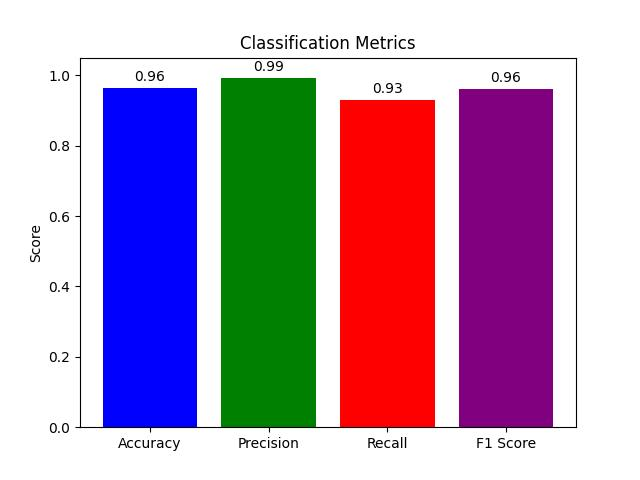
\includegraphics[scale=0.8]{./figures/metrics/experiment1English/classificationMetrics.jpg}
	\caption{Classification Metrics First Experiment}
	\label{classificationMetricsFirstExperiment}
\end{figure}

The Confusion Matrix provides a visual confirmation of the model's performance, with a high number of true positives (891) and true negatives (969), and relatively few false positives (6) and false negatives (67) \ref{confusionMatrixFirstExperiment}. This suggests the model has more problems when finding depression.

\begin{figure}[htbp]
	\centering
		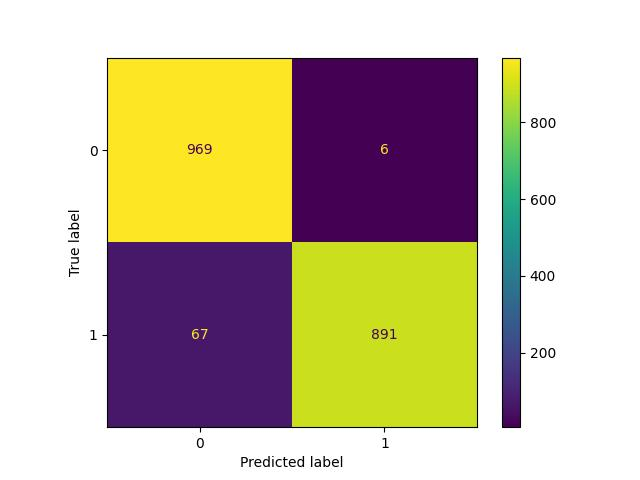
\includegraphics[scale=0.8]{./figures/metrics/experiment1English/confusionMatrix.jpg}
	\caption{Confusion Matrix First Experiment}
	\label{confusionMatrixFirstExperiment}
\end{figure}

Looking at the ROC Curve, the model demonstrates an excellent ability to distinguish between the classes, as evidenced by the area under the curve (AUC) being close to 1 (0.99) \ref{rocCurveFirstExperiment}. This suggests that the model has a good discrimination capability with a high true positive rate and a low false positive rate across different thresholds.

\begin{figure}[htbp]
	\centering
		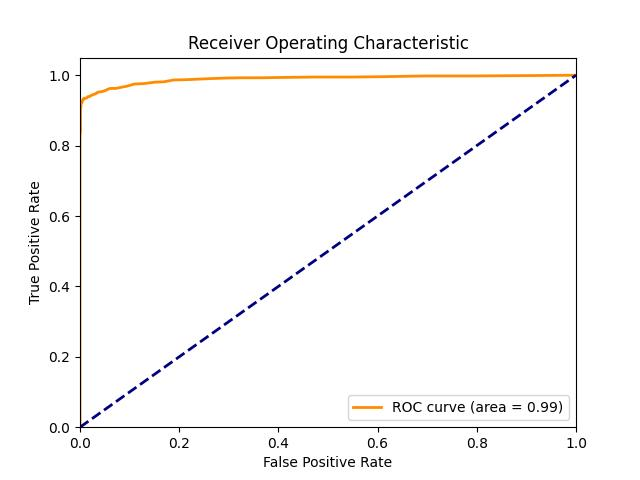
\includegraphics[scale=0.8]{./figures/metrics/experiment1English/roc_curve.jpg}
	\caption{ROC Curve First Experiment}
	\label{rocCurveFirstExperiment}
\end{figure}

The Top 10 Feature Importances plot indicates which features have the most influence on the model's predictions. The leading features, labeled as 'WC' (Word Count) and 'WPS' (Words per Sentence), seem to be the most significant drivers, with the others contributing to varying lesser degrees \ref{top10FeaturesFirstExperiment}. This shows that the length of the given text is very important in order for the model to give an accurate prediction.

\begin{figure}[htbp]
	\centering
		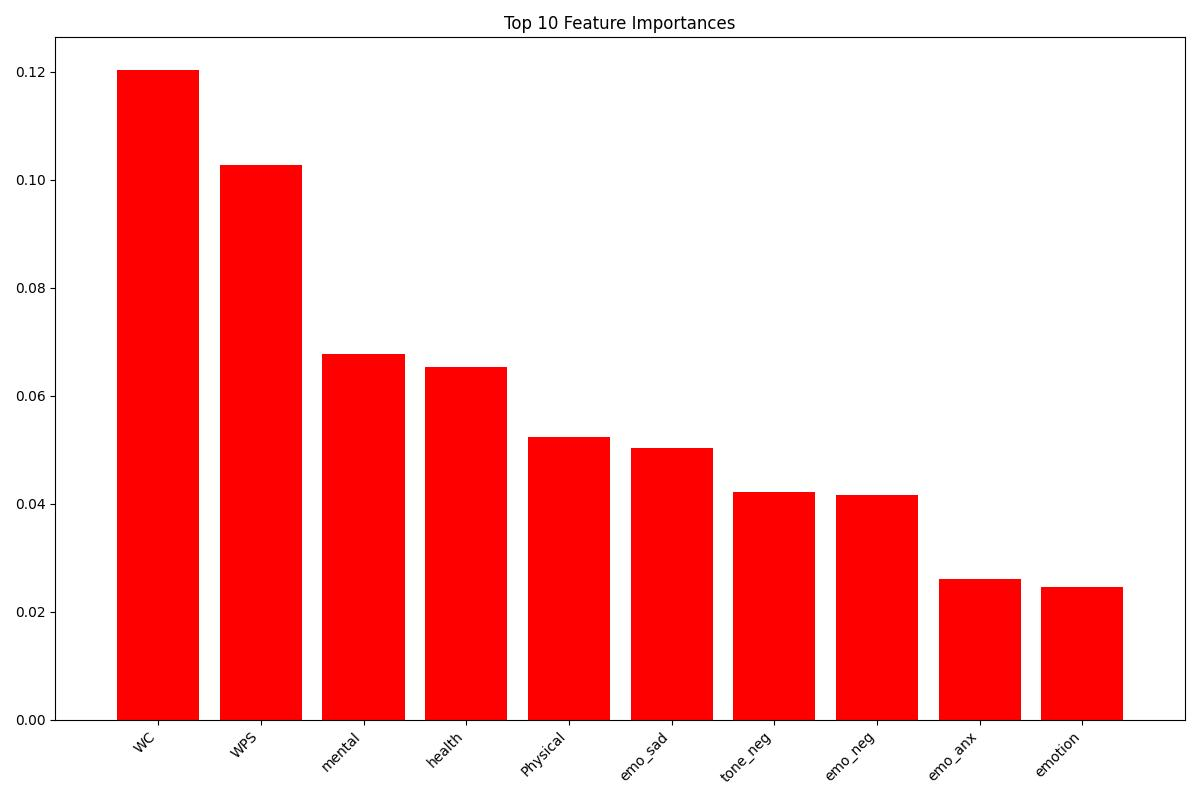
\includegraphics[scale=0.5]{./figures/metrics/experiment1English/top10features.jpg}
	\caption{Top 10 Feature Importances First Experiment}
	\label{top10FeaturesFirstExperiment}
\end{figure}

Overall, the model appears to be highly effective, with strong performance indicators, which seems to be the result of the analysis done for choosing the pre-processing methods and classifier, namely LIWC \cite{boyd2022development} and Random Forrest.

\subsection{Hyperparameter Tuning}
The selection of Random Forest hyperparameters is guided by the study \cite{probst2019hyperparameters}. The adjusted hyperparameters are:

\begin{itemize}
  \item \textbf{mtry}: This represents the number of features considered for splitting at each node. Lower values promote tree diversity and are beneficial when there are many relevant predictors. Given the large feature set, a value lower than the default square root of the number of features is suggested to prevent dominant features from overshadowing others.
  \item \textbf{Number of Trees}: A sufficient number of trees ensures stable predictions and importance estimates. While more trees generally improve model performance, beyond a certain point the marginal gains diminish. For practical purposes, between 500 to 1000 trees are recommended.
  \item \textbf{Node Size}: The node size controls the depth of the tree. Smaller node sizes can potentially lead to over-fitting, particularly when the number of features is high. A larger than 1 node size is preferred to mitigate this risk and improve computational efficiency.
  \item \textbf{Sample Size}: The proportion of data used for training each tree. Smaller sample sizes lead to more diversity but can decrease individual tree accuracy. Optimal sample size needs to be problem-specific but sampling a subset, such as between 20\% and 90\% of the data, can yield good results while reducing runtime. 
\end{itemize}

These hyperparameters were tuned using Sequential Model-Based Optimization (SMBO) to determine their optimal values while considering the Area Under the ROC Curve (AUC) as the performance metric \cite{probst2019hyperparameters}.

For the depression binary classifier multiple configurations were tested. It was noticed that the optimal ranges for the hyperparameters were:
\begin{itemize}
    \item \textbf{mtry}: between 6 and 10
    \item \textbf{Number of trees}: between 700 and 1000
    \item \textbf{Node Size}: between 3 and 9
    \item \textbf{Sample size}: between 6 and 9
\end{itemize}

After training with all combinations of the mentioned ranges, the one who got the best results was 6 for mtry, 900 for number of trees, 3 for node size and 8 for sample size. The same metrics as in the first experiment were used to analyze the performance of the model and improvements were seen. For the classification metrics accuracy(0.97) has improved by 0.01, precision stayed the same, recall(0.96) was the one who improved the most by 0.03, and F1-score(0.97) improved by 0.01. These values can be seen comparing Figure \ref{classificationMetricsFirstExperiment}, which shows the classification metrics for the first experiment, with Figure \ref{classificationMetricsSecondExperiment}, which shows them for the second experiment. This shows that because of hyperparameters tuning, it succeeded in improving the part where the model from the first experiment lacked.

\begin{figure}[htbp]
	\centering
		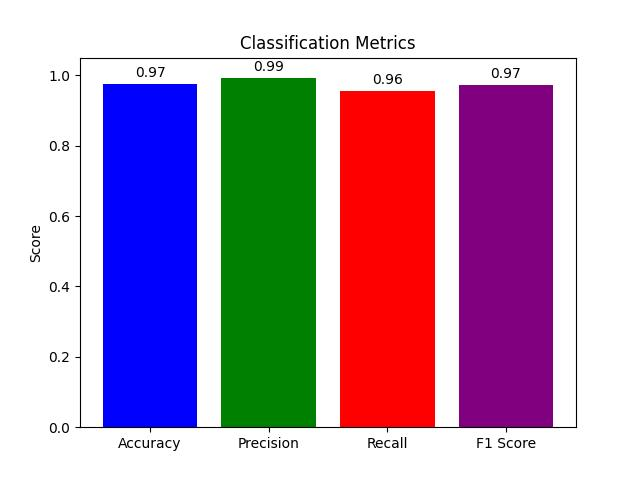
\includegraphics[scale=0.8]{./figures/metrics/experiment2English/classificationMetrics.jpg}
	\caption{Classification Metrics Second Experiment}
	\label{classificationMetricsSecondExperiment}
\end{figure}

In the case of the confusion matrix for the second experiment \ref{confusionMatriSecondExperiment} it can be discovered that in comparison with the one for the first experiment \ref{confusionMatrixFirstExperiment}, as can the improvement of recall also tell, the values of the false positives decreased, from 67 to 43.

\begin{figure}[htbp]
	\centering
		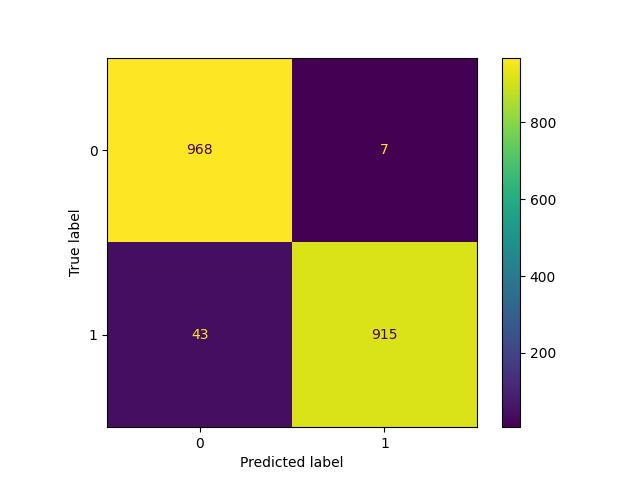
\includegraphics[scale=0.8]{./figures/metrics/experiment2English/confusionMatrix.jpg}
	\caption{Confusion Matrix Second Experiment}
	\label{confusionMatriSecondExperiment}
\end{figure}

For the ROC curve for this experiment \ref{rocCurveSecondExperiment}, the area stayed the same when looking to the first two digits, but an improvement of the true positive rate can be noticed from the initial experiment \ref{rocCurveFirstExperiment}.

\begin{figure}[htbp]
	\centering
		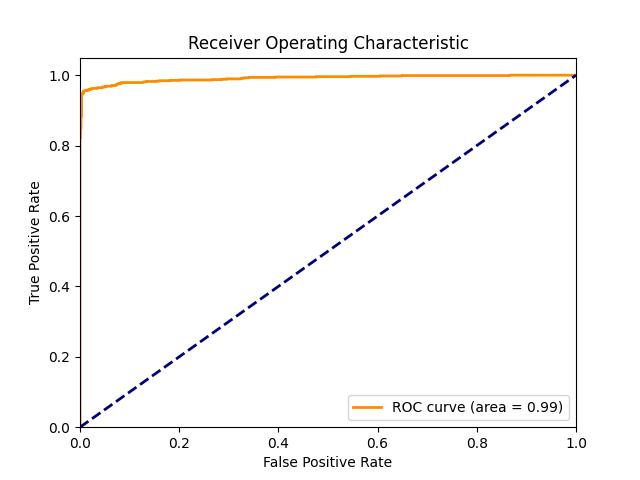
\includegraphics[scale=0.8]{./figures/metrics/experiment2English/roc_curve.jpg}
	\caption{ROC Curve Second Experiment}
	\label{rocCurveSecondExperiment}
\end{figure}

Seeing the top 10 features of the second experiment \ref{top10FeaturesSecondExperiment}, it was noticed that in comparison with the initial one \ref{top10FeaturesFirstExperiment} that even though WC (Word Count) and WS (Words per Sentence) are the still the most important features, they are now by much less, from 0.12 and 0.10 to both being at 0.09. This shows that now there are more features taken into account when the model makes the classification and each is more influential. Also it is remarked that a feature in the first ten was changed, namely emo\_anx (anxiety) with cause (causation).

\begin{figure}[htbp]
	\centering
		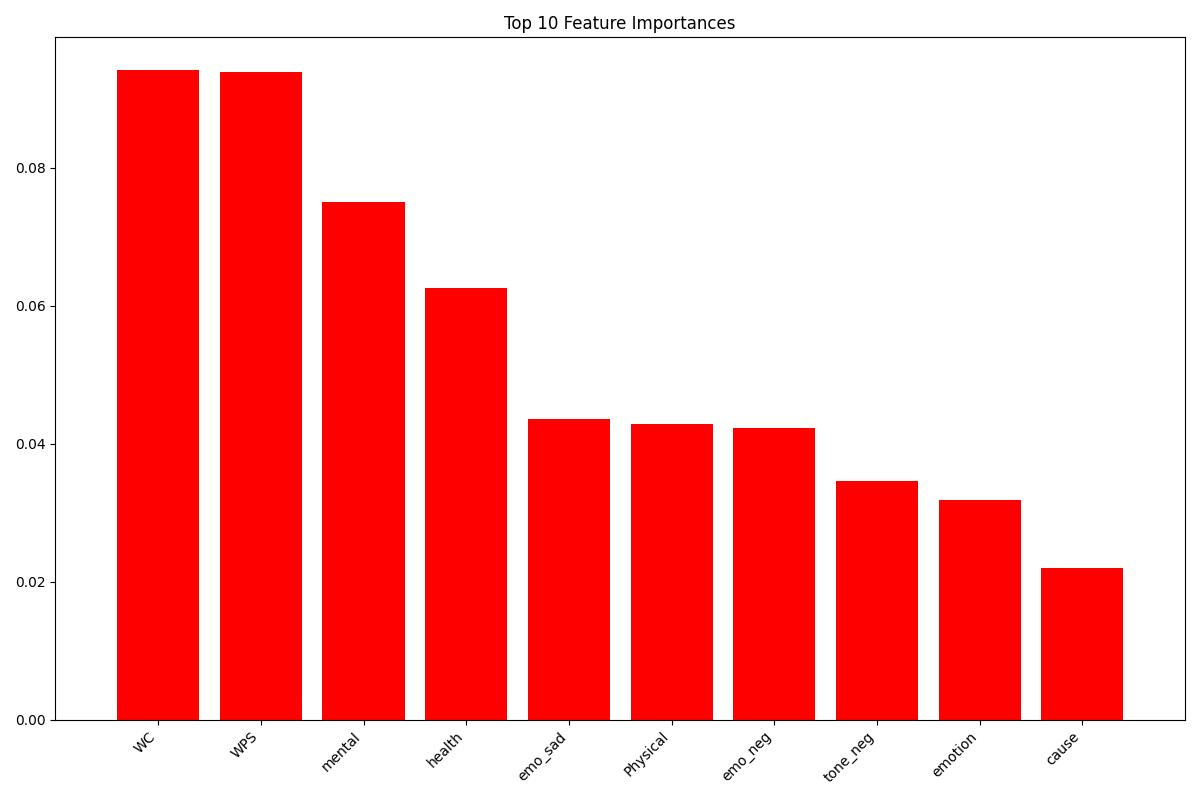
\includegraphics[scale=0.5]{./figures/metrics/experiment2English/top10features.jpg}
	\caption{Top 10 Feature Importances Second Experiment}
	\label{top10FeaturesSecondExperiment}
\end{figure}

\section{AI Model for Romanian Language}

\quad For the Romanian language model, the methodology was replicated consistently. The dataset was translated using "googletrans" Python library \cite{googletranslib} and LIWC served as the tool for preprocessing the data. However, the most recent English dictionary for LIWC-22 has not been translated into Romanian. The latest available version for Romanian is the LIWC-2015 dictionary, which contains only 86 features, compared to the 119 features available in the English version.

The training approach was aligned with the methodology used for the English model during the second experiment. The hyperparameters and the proportion of training to testing data remain consistent:

\begin{itemize}
\item \textbf{train/test split}: Maintained at 75/25, using stratification based on the 'is\_depression' label
\item \textbf{mtry}: 6
\item \textbf{Number of trees}: 900
\item \textbf{Node Size}: 3
\item \textbf{Sample size}: 8
\end{itemize}

This methodology facilitates a direct comparison between the performance of the Romanian and English models, ensuring consistent evaluation criteria across both. The same metrics were used for analysis. In terms of classification metrics, the most notable discrepancy arises in recall, where the Romanian model scores 0.87, falling short of the English model's 0.96 by 9 percentage points. Additionally, both accuracy and the F1-score have diminished by 0.05, while precision experienced the least impact, decreasing from 0.99 to 0.97. These metrics are illustrated in Figure \ref{classificationMetricsSecondExperiment} for the English model and in Figure \ref{classificationMetricsRomanianExperiment} for the Romanian model.

The diminished recall in the Romanian model suggests it is less adept at identifying true positive cases as compared to the English model. This lower performance may come from the nuances lost during the translation of the dataset from English to Romanian using the Googletrans library \cite{googletranslib}. Such translation challenges could contribute to the model’s reduced effectiveness, highlighting the influence of linguistic or cultural differences on the model’s ability to generalize across languages. The smaller reductions in accuracy and F1-score indicate that while the model is somewhat less effective overall, it still maintains a reasonable level of precision.

\begin{figure}[htbp]
	\centering
		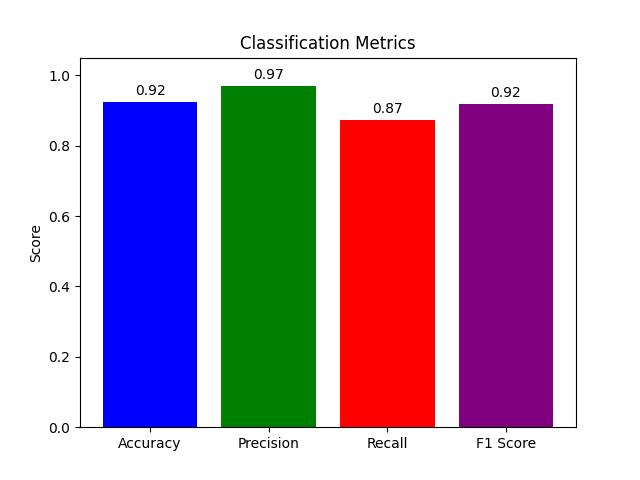
\includegraphics[scale=0.8]{./figures/metrics/experimentRomanian/classificationMetrics.jpg}
	\caption{Classification Metrics Romanian Model}
	\label{classificationMetricsRomanianExperiment}
\end{figure}

The confusion matrix \ref{confusionMatrixRomanianExperiment} illustrates a significant increase in false positives, rising from 43 in the English model \ref{confusionMatriSecondExperiment} to 123 in the Romanian model. However, the rise in false negatives was less marked, increasing from 7 to 26.

\begin{figure}[htbp]
	\centering
		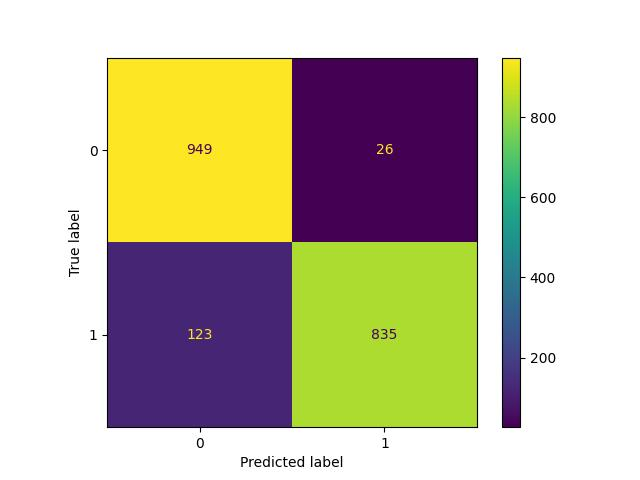
\includegraphics[scale=0.8]{./figures/metrics/experimentRomanian/confusionMatrix.jpg}
	\caption{Confusion Matrix Romanian Model}
	\label{confusionMatrixRomanianExperiment}
\end{figure}

Regarding the ROC curve, the Area Under the Curve (AUC) experienced a slight decrease of 0.01, as depicted in Figure \ref{rocCurveRomanianExperiment} compared to Figure \ref{rocCurveSecondExperiment}. These metrics collectively indicate that the issues observed during the experimentation with the English model are more pronounced in the Romanian classifier.

\begin{figure}[htbp]
	\centering
		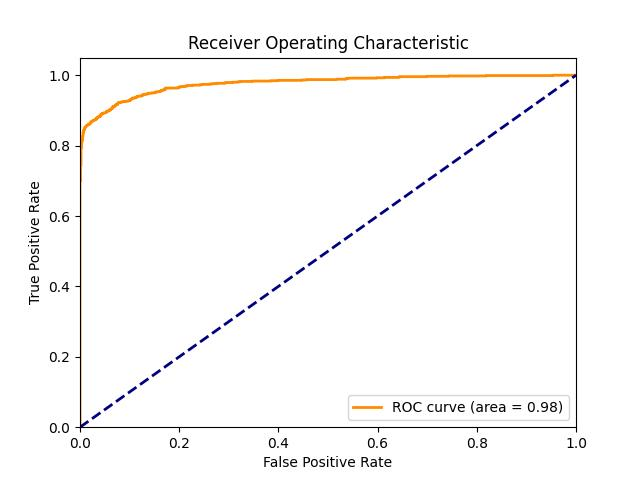
\includegraphics[scale=0.8]{./figures/metrics/experimentRomanian/roc_curve.jpg}
	\caption{ROC Curve Romanian Model}
	\label{rocCurveRomanianExperiment}
\end{figure}

The most significant features for the Romanian classifier \ref{top10FeaturesRomanianExperiment} align more closely with those observed in the initial experiment for the English model \ref{top10FeaturesFirstExperiment}. Notably, Word Count (WC) has risen above 0.12, surpassing the prominence it held in the first experiment. This contrasts with the enhancements seen in the second English experiment \ref{top10FeaturesSecondExperiment}, where a diminished reliance on WC and WPS (Words per Sentence) indicated a broader array of features influencing the English classifier’s decisions. However, this diversification does not appear to extend to the Romanian model.

Some features remain consistent with the English LIWC-22 dictionary features listed in the top 10 for the second experiment; for instance, "sad" aligns with "emo\_sad", and both "cause" and "health" are both present and "negemo" is the same as "emo\_neg". The "anx" feature mirrors "emo\_anx" from the first experiment’s top features. The presence of "Period" suggests that the Googletrans library has introduced punctuation marks, which have become a significant element. The evolution from LIWC-2015 to LIWC-22 is further evidenced by the removal of the "interrog" category in the Romanian model’s top 10 features, which was dropped in LIWC-22 due to its low base rates, internal reliability, or infrequent usage, as noted in \cite{boyd2022development}. The "ipron" feature might also result from the machine translation process.

\begin{figure}[htbp]
	\centering
		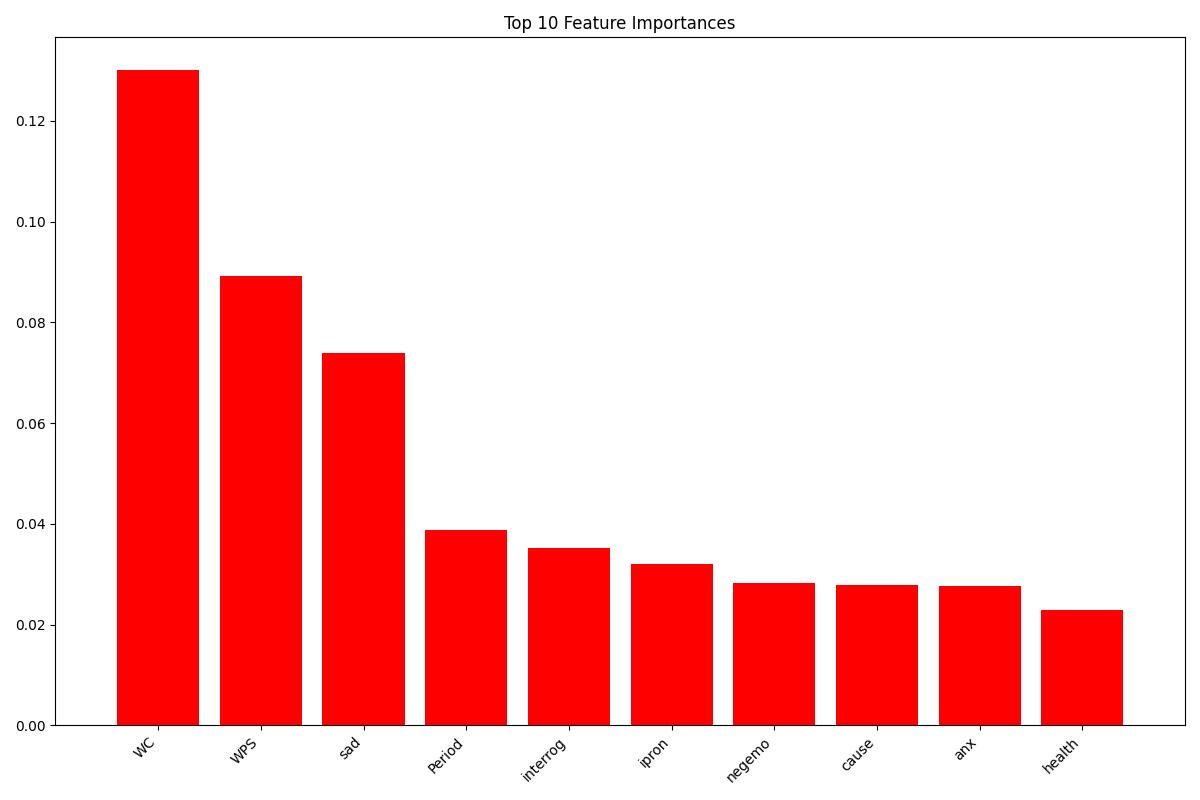
\includegraphics[scale=0.5]{./figures/metrics/experimentRomanian/top10features.jpg}
	\caption{Top 10 Features Romanian Model}
	\label{top10FeaturesRomanianExperiment}
\end{figure}

\section{Discussion}\label{discussion}
This chapter gives a SWOT analysis of the proposed model.
\begin{itemize}

\item{\textbf{Strengths}:The English model showed better performance than the Romanian one, due to LIWC-22 being only in English, meaning that translating input text from any language to English may show reliable results.}

\item{\textbf{Opportunities}: The model can be used in order to prevent severe symptoms of depression through analysing a company's web application text or even employees messages or posts. It could also greatly aid in targeted marketing for psychologists or enhancing mental health awareness.}

\item{\textbf{Weaknesses}: LIWC \cite{boyd2022development} specifies its use strictly for academic purposes, any commercial application would need to adopt a different pre-processing approach. Also a professional psychologist is needed in order to give a human-based assesment.}

\item{\textbf{Threats}: Due to the information being processed by the model being sensitive, security is very important in the process of parsing input from the an application's frontend.}
     
\end{itemize}
\section{Conclusions and future work}\label{conclusions}

\quad Developing a multilingual tool presents significant challenges. There is a much richer body of literature for English than for Romanian, which impacts the performance of AI models, as showed by the experiments. The English model achieved a precision of 96\%, significantly higher than the Romanian model's 87\%. This difference largely comes from the translation methods used and the limitations of the pre-processing tool LIWC. Despite using Google Translate, a leading translation service, the Googlelib \cite{googletranslib} encountered difficulties in maintaining the original text's meaning. Additionally, the most recent version of LIWC, LIWC-22, is only available in English, which meant a downgrade to LIWC-2015 for Romanian, which is seven years behind in advancements, as reflected in the precision of the Romanian classifier.

For future improvements, employing an AI-based translation tool could preserve text meaning more effectively. The next step for the tool is its deployment to a production environment, transitioning from localhost to a cloud hosting platform to ensure broader accessibility and reliability.

Moreover, while communicating, words represent only a minor fraction of the information conveyed. The tool, which solely analyzes text, is insufficient to conclusively determine if a person is depressed. Therefore, it is important to note that the tool serves merely as a preliminary assessment of a person’s emotional state, a thorough evaluation requires a professional in psychology. For a more accurate computer-based analysis, it would be necessary to consider all aspects of communication, both verbal and nonverbal.



\footnotesize{

\bibliographystyle{elsarticle-harv}
\bibliography{biblio}
\null


} 

\end{document}

%%
%% End of file `Sample Paper.tex'.
